\section{实验结果}

\subsection{超参数$\omega$的影响}
\label{sec:4_omega}
本章提出的多任务训练方法包含了翻译和CER两个由超参数$\omega$控制训练比例的任务,而CER又包含了TER、VER和TNER三个由$\alpha$、$\beta$和$\gamma$三个超参数控制的子任务。因此如何平衡这些任务的训练比重是在模型训练过程中极为重要的问题。本章根据三个子任务的重要程度,将$\alpha$、$\beta$和$\gamma$三个超参数的比例固定为$2:2:1$,然后通过调节超参数$\omega$来寻找翻译和CER两个任务合适的训练比例。本节依据CER-NMT在英德翻译验证集上的BLEU值结果来选取一个合适的$\omega$值。

%\begin{figure}[!htbp]
%    \centering
%    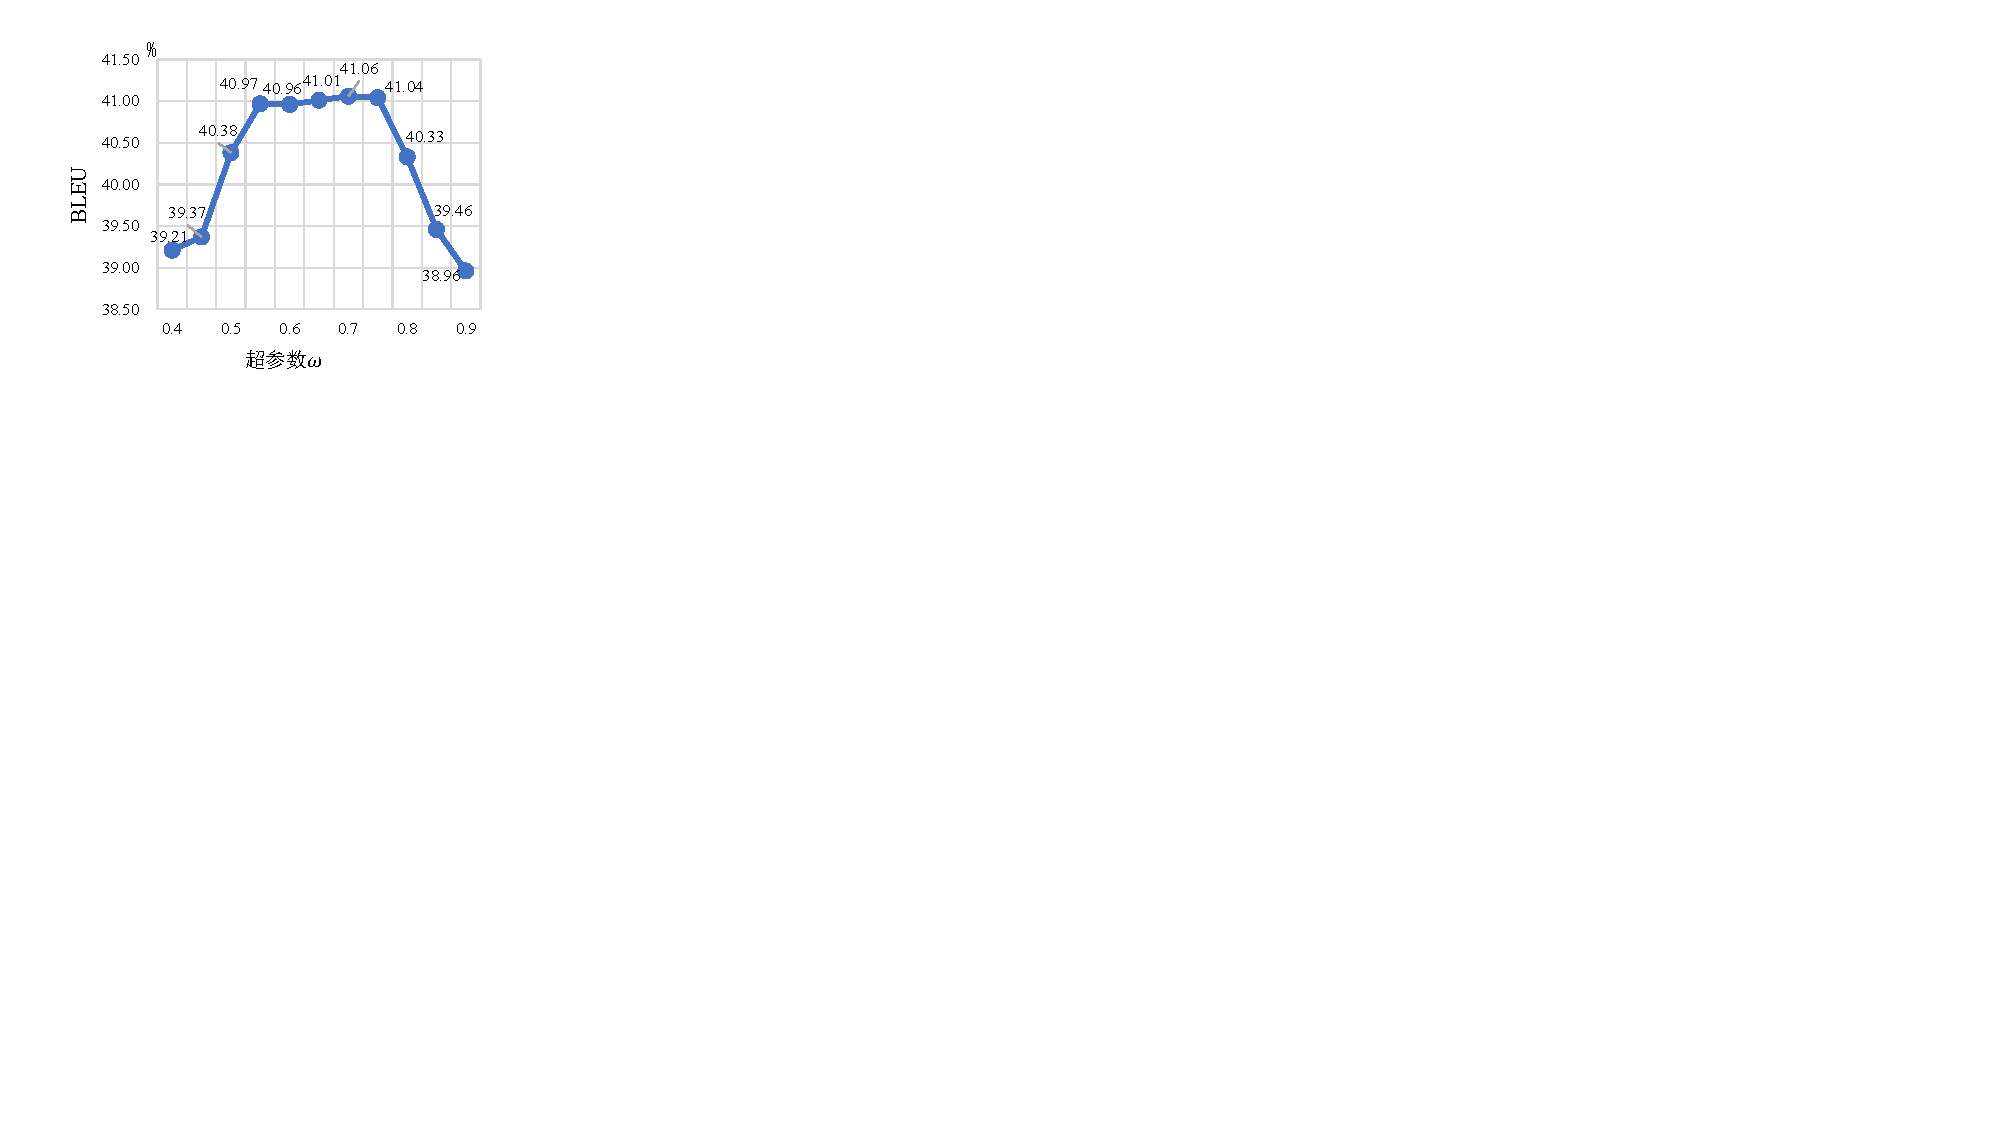
\includegraphics[scale=1.2]{Img/fig_4_searchw.pdf}
%    \bicaption{超参数$\omega$对CER-NMT翻译准确率的影响}{Effect of hyperparameter $\omega$ on translation accuracy of CER-NMT}
%    \label{fig:4_searchw}
%\end{figure}


\begin{figure}[!htbp]
    \centering
    \begin{subfigure}[b]{0.5\textwidth}
      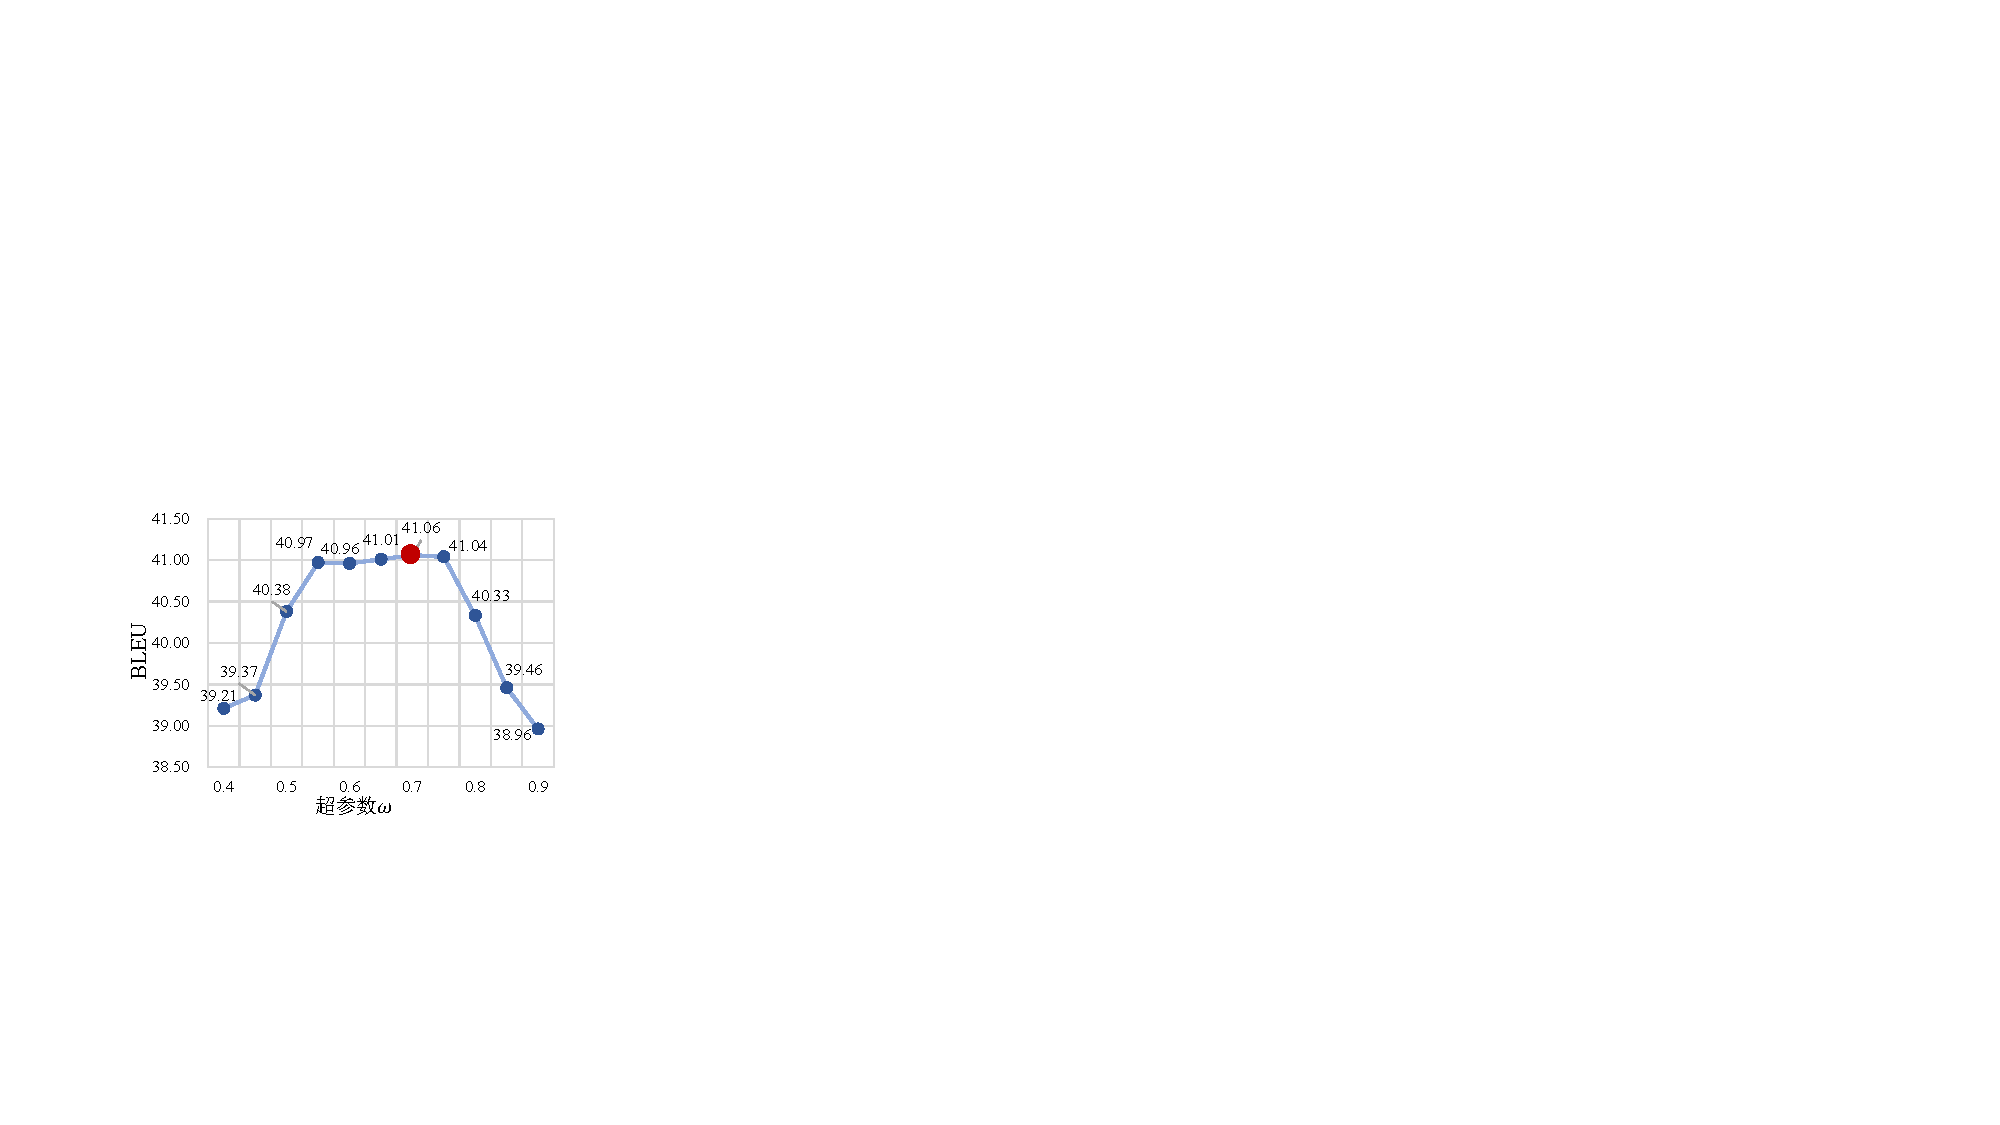
\includegraphics[width=\textwidth]{Img/fig_4_searchw_ende.pdf}
      \caption{英德翻译}
      \label{fig:4_searchw_ende}
    \end{subfigure}%
    ~% add desired spacing
    \begin{subfigure}[b]{0.5\textwidth}
      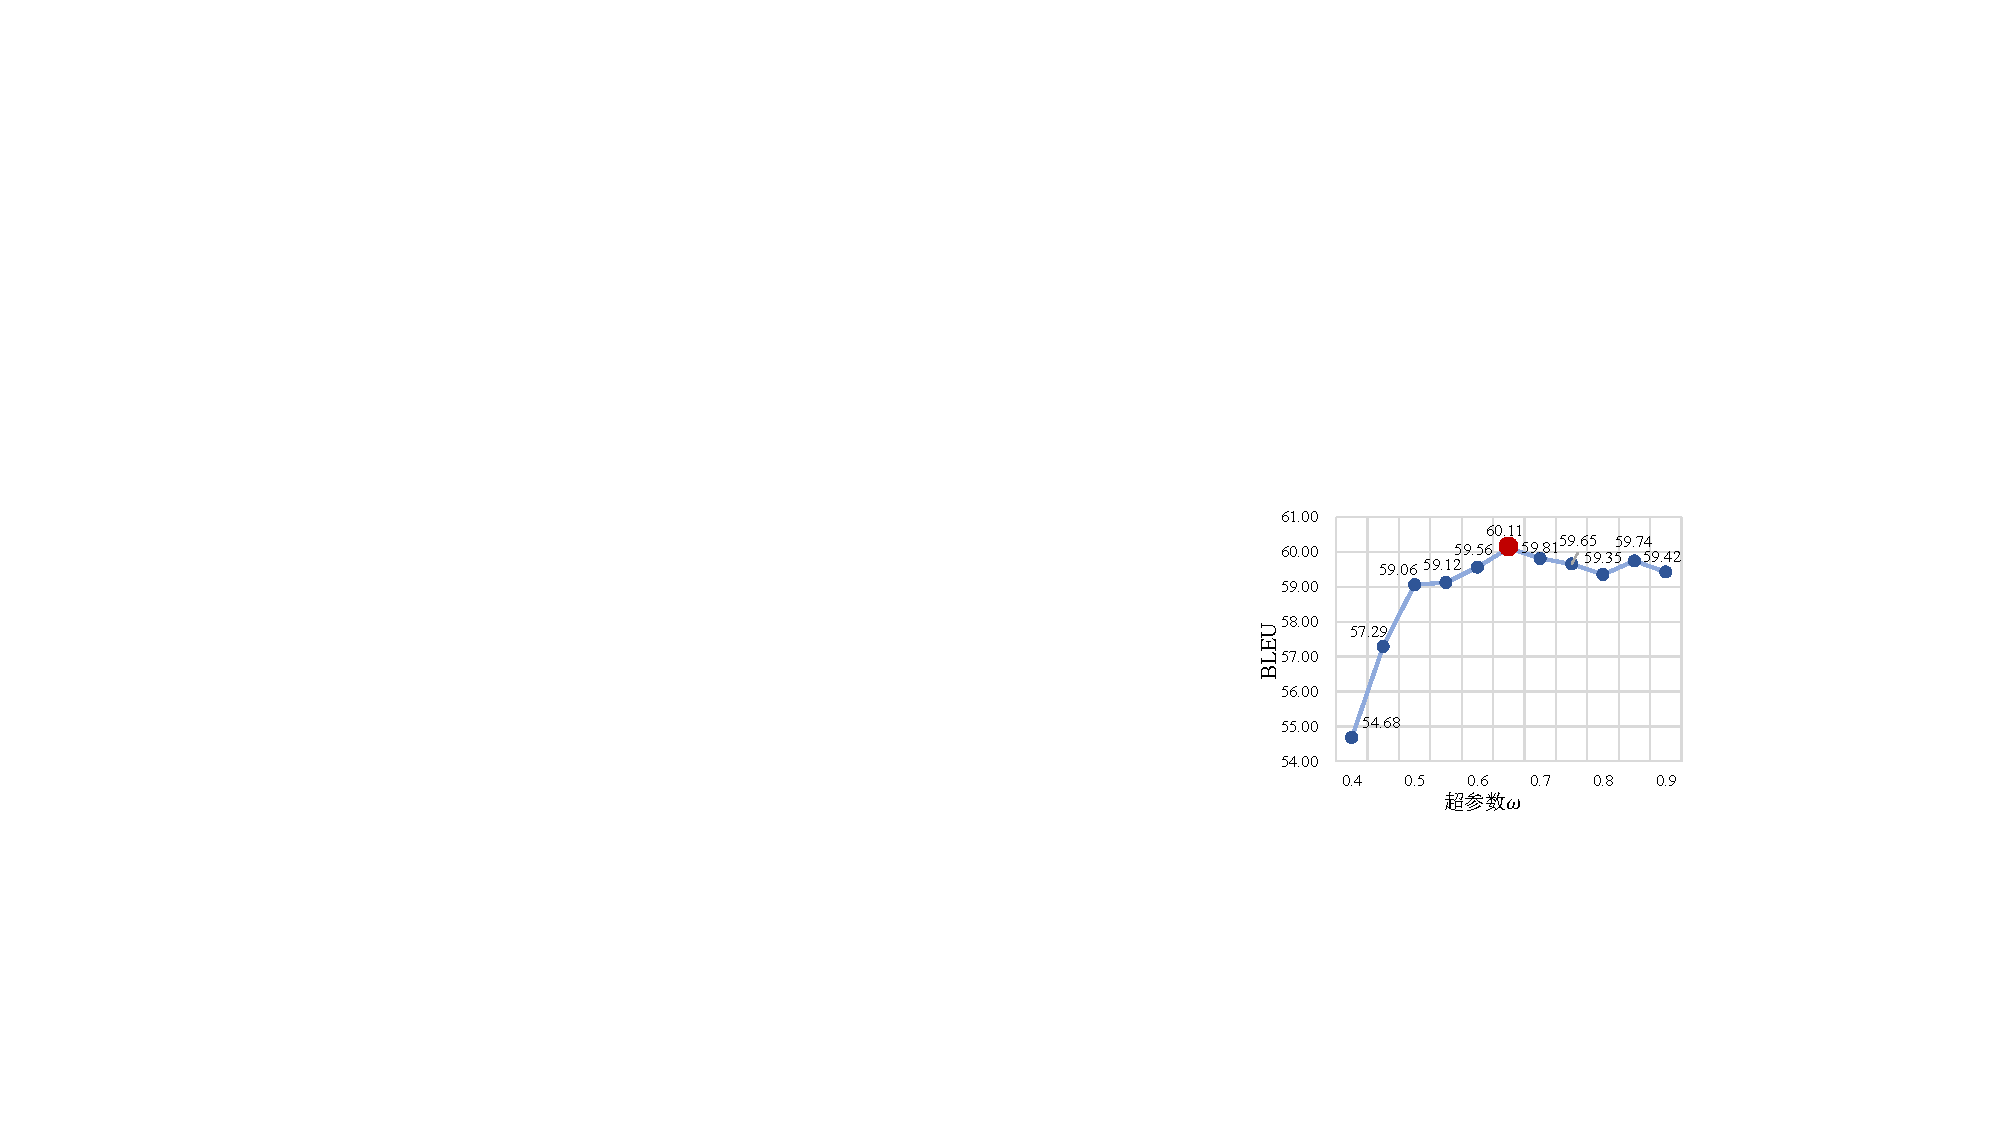
\includegraphics[width=\textwidth]{Img/fig_4_searchw_enfr.pdf}
      \caption{英法翻译}
      \label{fig:4_searchw_enfr}
    \end{subfigure}
    \\% line break
    \begin{subfigure}[b]{0.5\textwidth}
      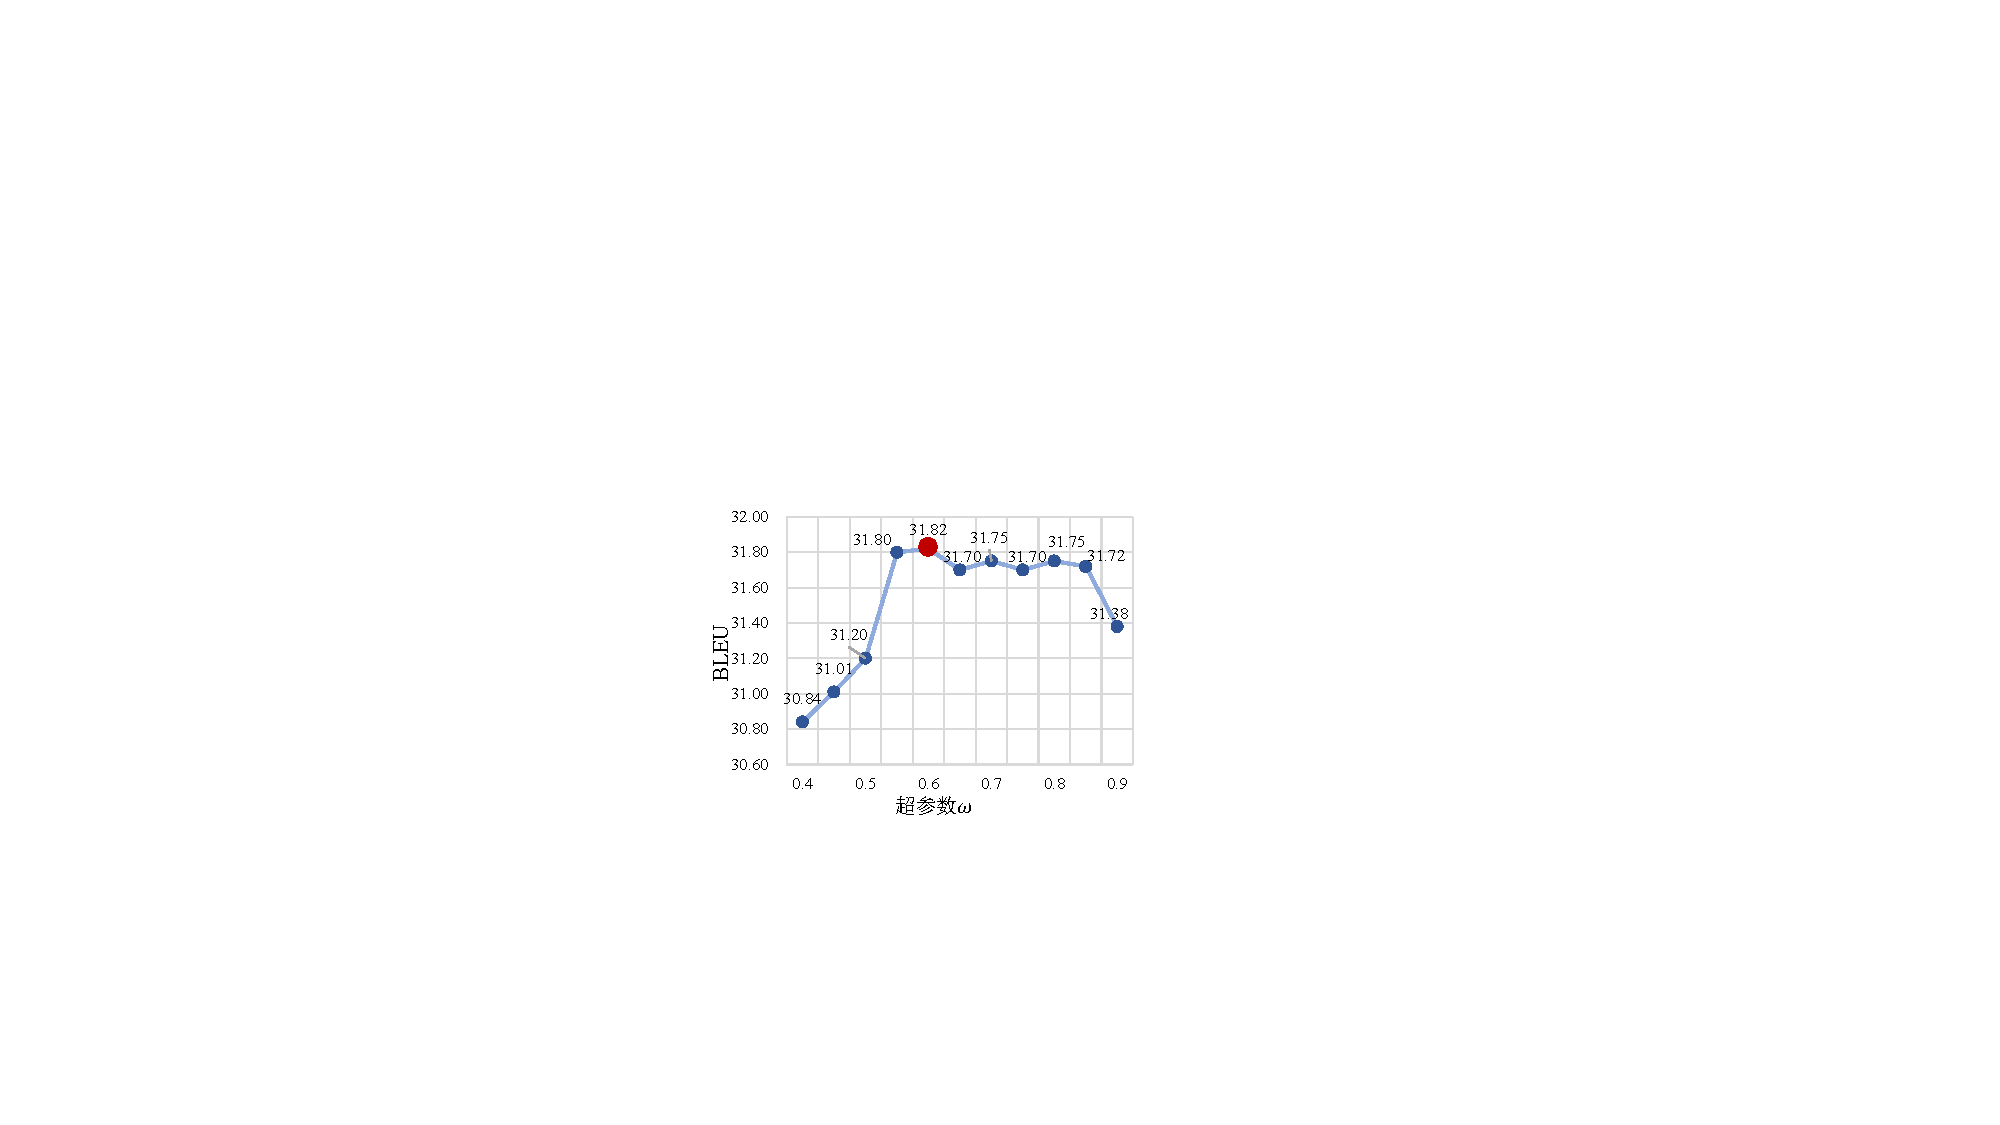
\includegraphics[width=\textwidth]{Img/fig_4_searchw_encs.pdf}
      \caption{英捷翻译}
      \label{fig:4_searchw_encs}
    \end{subfigure}%
    \bicaption{超参数$\omega$对CER-NMT翻译准确率的影响}{Effect of hyperparameter $\omega$ on translation accuracy of CER-NMT}
    \label{fig:4_searchw}
\end{figure}
如图\ref{fig:4_searchw}所示实验结果,横轴代表$\omega$从0.4以0.05为间隔增加至0.9,纵轴为NMT模型在英译德验证集上的BLEU值。当$\omega=1.0$时,代表翻译任务的训练比例为$100\%$,此时是纯文本神经机器翻译。当$\omega=0.0$时,代表仅训练CER不做翻译。该图反映出,当$\omega \in [0.5,0.8]$时,模型均具有较好的效果。超过这个范围时,CER-NMT的BLEU值将逐渐接近纯文本翻译模型。低于这个范围时,CER-NMT的翻译准确率发生了骤减。我们还测试了当$\omega=0.3$时的情况,此时BLEU值以骤减到9.86。以上实验结果说明在一个合适的范围内,CER方法能够帮助翻译模型提升翻译准确率。而这个范围应当使模型的训练过程主要以翻译任务为主以CER为辅。因此,本章选择$\omega=0.7$,即CER-NMT在验证集上达到最高的BLEU值时,作为后续试验中对超参数$\omega$的设置。


\subsection{翻译结果}
\label{sec:4_ende}


\begin{table}[!htbp]
    \bicaption{在Multi30K英德翻译上的结果。}{Translation results on Multi30K EN-DE.}
    \label{tab:4_ende_enfr}
    \centering
    \footnotesize% fontsize
    \setlength{\tabcolsep}{4pt}% column separation
    \renewcommand{\arraystretch}{1.2}%row space 
\begin{tabular}{ccccccccc}
\hline
 \multirow{3}{*}{模型} & \multicolumn{6}{c}{英译德} & \multicolumn{2}{c}{英译法} \\
\cmidrule(r){2-7} \cmidrule(r){8-9}%\hline
       & \multicolumn{2}{c}{Test2016} & \multicolumn{2}{c}{Test2017} & \multicolumn{2}{c}{MSCOCO} & \multicolumn{2}{c}{Test2016} \\
\cline{2-9}%\cmidrule(r){2-7} \cmidrule(r){8-9} %\cline{2-9}
              &    BLEU & METEOR &     BLEU & METEOR &     BLEU & METEOR &     BLEU & METEOR \\
\hline
\multicolumn{9}{c}{图片信息辅助式方法} \\
\hline
SerialAtt      & 38.7 & 57.2 & - & - & - & - & 60.8 & 75.1 \\
DelMMT           & 38.0 & 55.6 & - & - & - & - & 59.8 & 74.4 \\
GAMMT      & 39.2 & {\textbf{57.8}} & 31.4 & 51.2 & 26.9 & 46.0 & - & - \\
GMMT             & 39.8 & 57.6 & 32.2 & 51.9 & 28.7 & {\textbf{47.6}} & 60.9 & 74.9 \\
\hline
\multicolumn{9}{c}{图片信息增强式方法} \\
\hline
Imagination      & 36.8 & 55.8 & - & - & - & - & - & - \\
ImagiT   & 38.6 & 55.7 & 32.1 & {\textbf{52.4}} & - & - & 59.9 & 74.3 \\
CTR-NMT             & 39.7 & 57.5 & {\textbf{32.9}} & 51.7 & {\textbf{29.1}} & 47.5 & 61.1 & 75.8 \\
\hline
\multicolumn{9}{c}{本章所提方法} \\
\hline
Transformer             & 38.5 & 57.5 & 31.0 & 51.9 & 27.5 & 47.4 & 60.5 & 75.6 \\
CER-NMT          & {\textbf{40.2}} & {\textbf{57.8}} & 32.5 & 52.0 & 28.3 & 47.1 & {\textbf{61.6}} & {\textbf{76.1}} \\
\bottomrule
\end{tabular}
\end{table}

表\ref{tab:4_ende_enfr}显示了采用了CER方法的NMT系统的翻译结果。其中$\omega$按照4.1节的结论取值为0.7,对应的VER、TER和TNER三个子任务的训练比重分别为$12\%$、$12\%$和$6\%$。


表\ref{tab:4_ende_enfr}中加粗项表示整列中的最佳结果。根据以上英译德和英译法的实验结果可以得到以下结论:

%\begin{itemize}
%\item
(1)本章所提方法在Multi30K Test2016测试集的英德翻译和英法翻译两种语言对上取得了BLEU和METEOR的最佳结果,并且在Test2017测试集上的结果超过了多数模型的结果,并与其它模型的最佳结果相比差距很小。这说明CER方法能够有效提升NMT模型的翻译质量。

%\item
(2)CER-NMT在歧义词较多的Ambiguous MSCOCO上的表现并不理想,落后于GMMT和上一章的CTR-NMT两个模型。这是因为CER方法主要帮助翻译模型在训练阶段融合视觉信息,在测试阶段因为不需要输入图像使得模型无法借助视觉信息解决歧义词的问题。同理可以看到,CTR-NMT在METEOR上的提升也仅有0.1。这说明图片信息增强式的方法虽然能够提升模型的翻译质量,但也同样具有一定的局限性。例如文本中常见的歧义词问题或语义不完整问题,是需要利用图片信息辅助翻译模型来解决。

(3)%\item
GMMT、CTR-NMT和CER-NMT均是采用视觉目标作为视觉输入的方法,其结果均优于采用完整图片输入的方法。理想的情况下,完整的图片包含的视觉信息更完整,对翻译带来的好处会更多。但是目前实验结果说明,在神经机器翻译中融合图片信息是非常困难的,需要为NMT模型提供更细粒度的视觉信息才能降低跨模态信息融合的难度,使模型更多地利用图片中的视觉信息。
%\end{itemize}

综合以上的实验结果,本章所提的跨模态实体重构方法能有效地提升机器翻译的质量。同时也说明了虽然图片信息增强式的翻译方法无法解决歧义词和语义不完整问题,但是方法的有效性也体现了图片信息具有除补全语以外的其它作用。

\subsection{消融实验}
\label{sec:4_ablation_study}
为了探究VER、TER和TNER三个子任务对CER$-$NMT模型的影响,本节设置了12组消融实验。其中序号0代表4.2节中CER-NMT的结果。序号1$-$3组各去掉一个子任务,并保持剩余子任务的训练权重。序号4$-$5组各去掉一个子任务,保持NMT的权重。序号7$-$9组各保留一个子任务,保持子任务的权重。序号10$-$12组保留一个子任务,保持NMT的权重。

\begin{table}[!htbp]
    \bicaption{在Multi30K Test2016英德翻译上消融实验}{Ablation study on the EN-DE of Multi30K Test2016}
    \label{tab:4_ablation_study}
    \centering
    \footnotesize% fontsize
    \setlength{\tabcolsep}{8pt}% column separation
    \renewcommand{\arraystretch}{1.2}%row space 
\begin{tabular}{cccccc}
\hline
\multirow{2}{*}{序号} & NMT & VER & TER & TNER & \multirow{2}{*}{BLEU} \\
\cline{2-5}
   & $\omega$ & $\omega \times \alpha$ & $\omega \times \beta$ & $\omega \times \gamma$ & \\
\hline
0  & 0.70 & 0.12 & 0.12 & 0.06 & 40.2 \\
\hline
1  & 0.76 & 0.12 & 0.12 &  -   & 40.0 \\
2  & 0.82 & 0.12 & -    & 0.06 & 39.5 \\
3  & 0.82 & -    & 0.12 & 0.06 & 39.6 \\
\hline
4  & 0.70 & 0.15 & 0.15 & -    & 39.9 \\
5  & 0.70 & 0.20 & -    & 0.10 & 39.2 \\
6  & 0.70 & -    & 0.20 & 0.10 & 39.3 \\
\hline
7  & 0.88 & 0.12 & -    & -    & 38.8 \\
8  & 0.88 & -    & 0.12 & -    & 38.8 \\
9  & 0.94 & -    & -    & 0.06 & 39.0 \\
\hline
10 & 0.70 & 0.30 & -    & -    & 39.2 \\
11 & 0.70 & -    & 0.30 & -    & 39.4 \\
12 & 0.70 & -    & -    & 0.30 & 39.0 \\
\hline
\end{tabular}
\end{table}

实验结果如表2所示,其中“-”代表所对应的子任务被去掉,可以获得如下信息:

%\begin{itemize}
%\item
(1)序号1$-$6组各去掉了一个子任务,序号7$-$12组各仅保留一个子任务。从两组之间的对比可以看出,1$-$3的结果整体优于7$-$8,4$-$6的结果整体优于10$-$12,说明无论是保持子任务的训练比重不变还是保持翻译任务的训练比重不变,子任务组合的方式总是优于仅使用单一的子任务。其中,VER和TER的在序号1和4中的组合已经可以使翻译模型得到很好的结果。TNER对NMT的影响最小,但是依旧可以为NMT模型带来小幅度的提升。

%\item
(2)$\omega>0.8$的实验组2,3,7,8,9的结果与\ref{sec:4_omega}小节中的实验结果均说明减少跨模态任务至一定比重后,模型的翻译准确率将逐渐趋近于纯文本翻译模型。

%\item
(3)与\ref{sec:4_ende}小节中CER-NMT的实验结果相比可以说明,针对实体重构的VER和TER任务对翻译模型的性能影响最大,且这两个任务组合情况下的结果要优于单独使用的情况。相比之下,TNER同样可以为翻译性能带来一定的提升,但效果不如实体重构明显。综合以上,TER、VER和TNER三个子任务共同配合可以使翻译模型的性能达到最佳。
%\end{itemize}


\subsection{文本实体忠实度}
\label{sec:4_fidelity}
本章所提方法对视觉实体与文本实体互相结合跨模态信息,再将视觉实体与文本上下文相融合。而这一过程中是以实体间的信息融合为主导的,\ref{sec:4_ablation_study}小节的实验也证实了这一点。这使得视觉信息具有明确的作用方向。因此检验视觉信息是否对文本实体的翻译产生了影响成为了一个必要的环节。本节我们将尝试测量在解码生成目标单词时对文本实体的忠实度来反映模型的行为变化。

Transformer的解码器采用的是交叉注意力机制,与一般的注意力机制类似的是,在解码过程中通过给源端的词不同的“权重”来达到“关注”或“忽视”的作用。该“权重”体现了当前要解码的目标端单词对源端单词所提供信息的需求程度。因此,我们选择Transformer解码器最后一层交叉注意力权重的多头平均值,作为生成目标端词时对源端词的注意力“权重”,并定义该“权重”为忠实度(Fidelity),用于量化生成目标端文本实体时对源端文本实体的忠实程度。\ref{sec:4_dataset}小节中提到,源端的文本实体是通过文本分析工具提取得到。本节中所要确定的目标端文本实体是通过fast-align\cite{45_dyer-etal-2013-simple}对齐工具对齐源端与目标端单词得到的。为了得到一个较好的对齐结果,我们将测试集与训练集拼接后训练对齐模型。


\begin{figure}[!htbp]
    \centering
    \begin{subfigure}[b]{0.5\textwidth}
      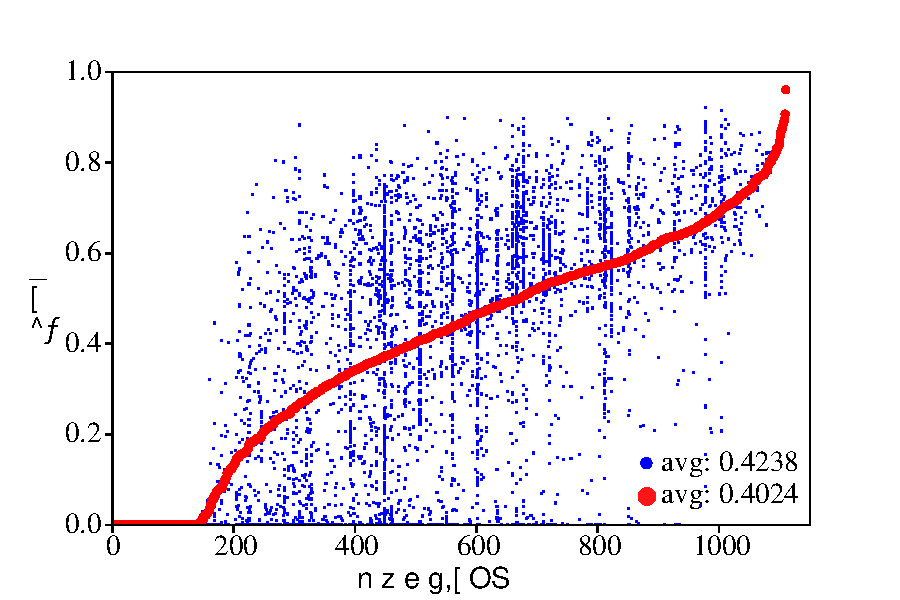
\includegraphics[width=\textwidth]{Img/fig_4_fidelity_base.pdf}
      \caption{Transformer}
      \label{fig:4_fidelity_base}
    \end{subfigure}%
    ~% add desired spacing
    \begin{subfigure}[b]{0.5\textwidth}
      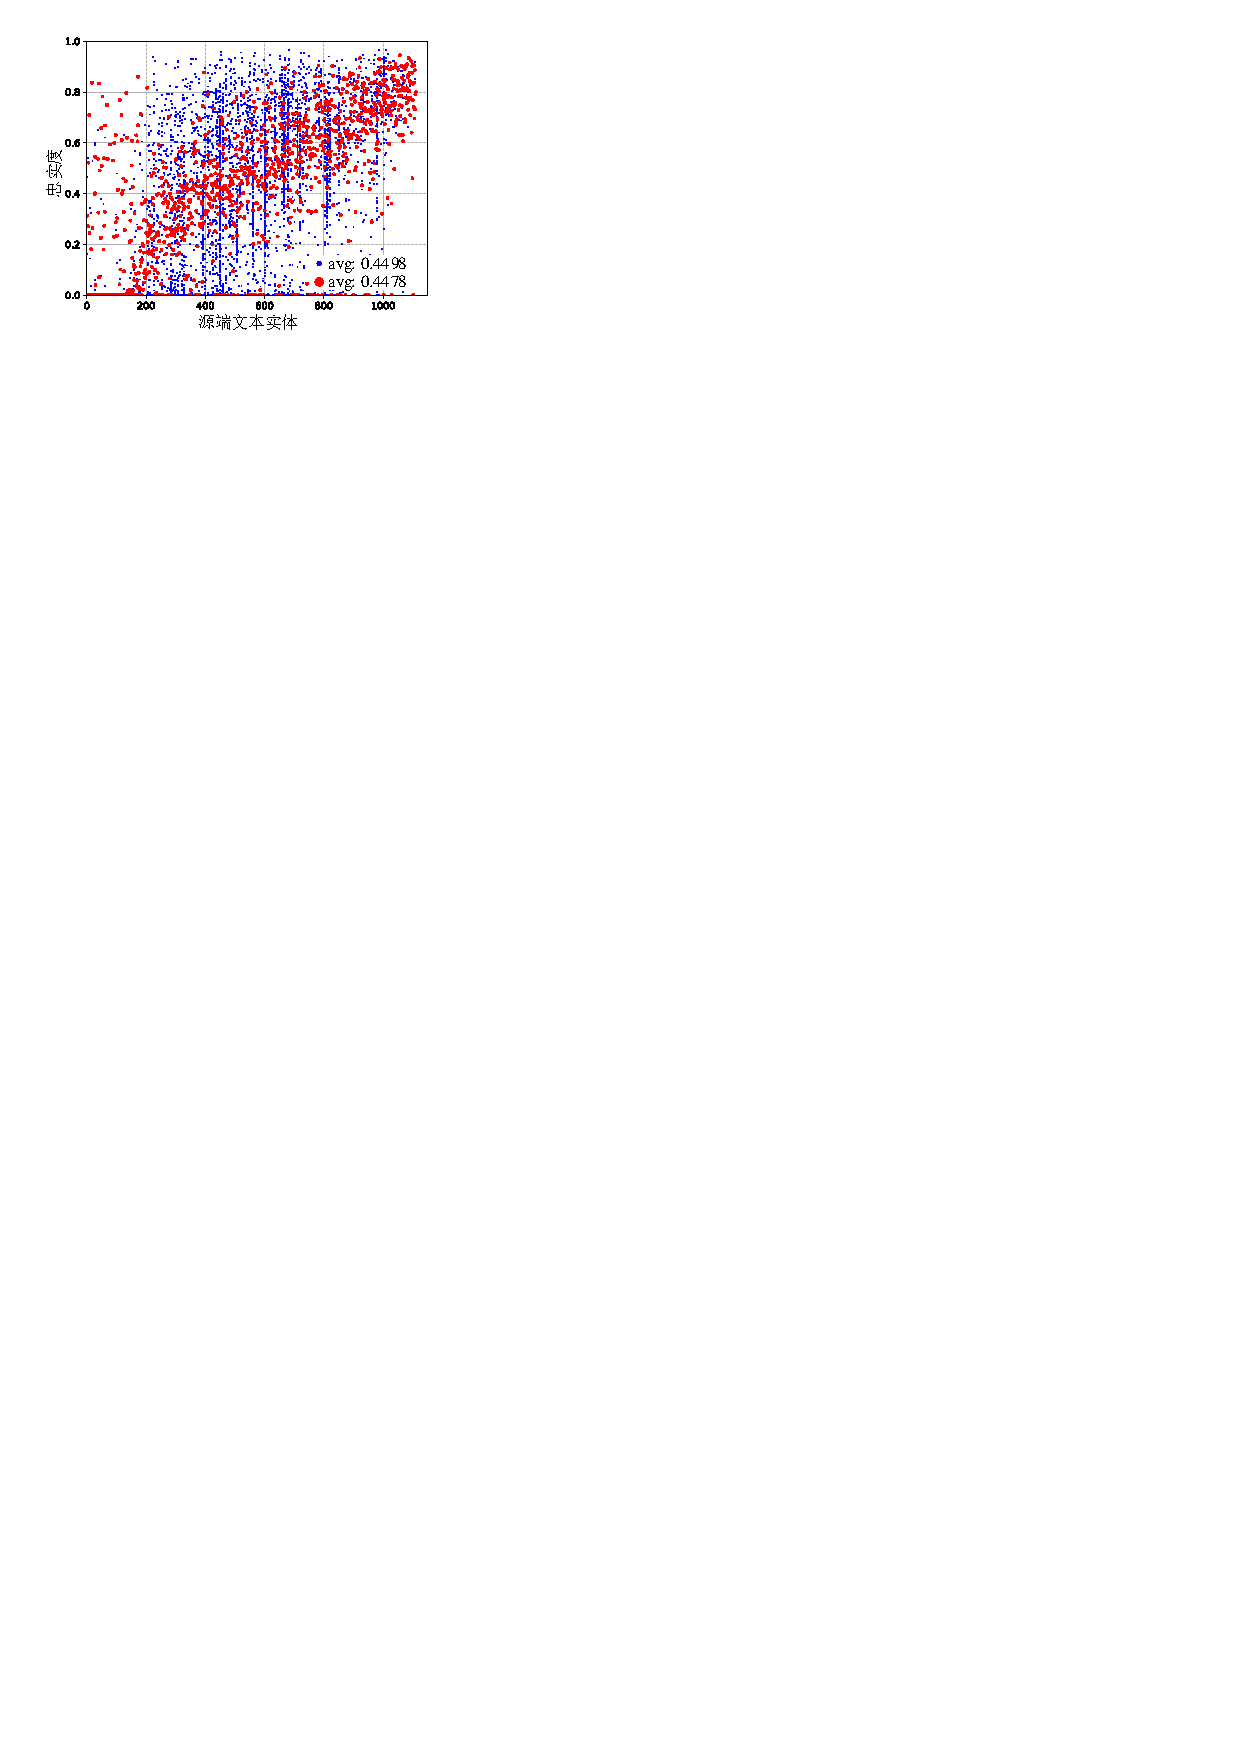
\includegraphics[width=\textwidth]{Img/fig_4_fidelity_cer_baseorder.pdf}
      \caption{CER-NMT}
      \label{fig:4_fidelity_cer_baseorder}
    \end{subfigure}
    \\% line break
    \begin{subfigure}[b]{0.5\textwidth}
      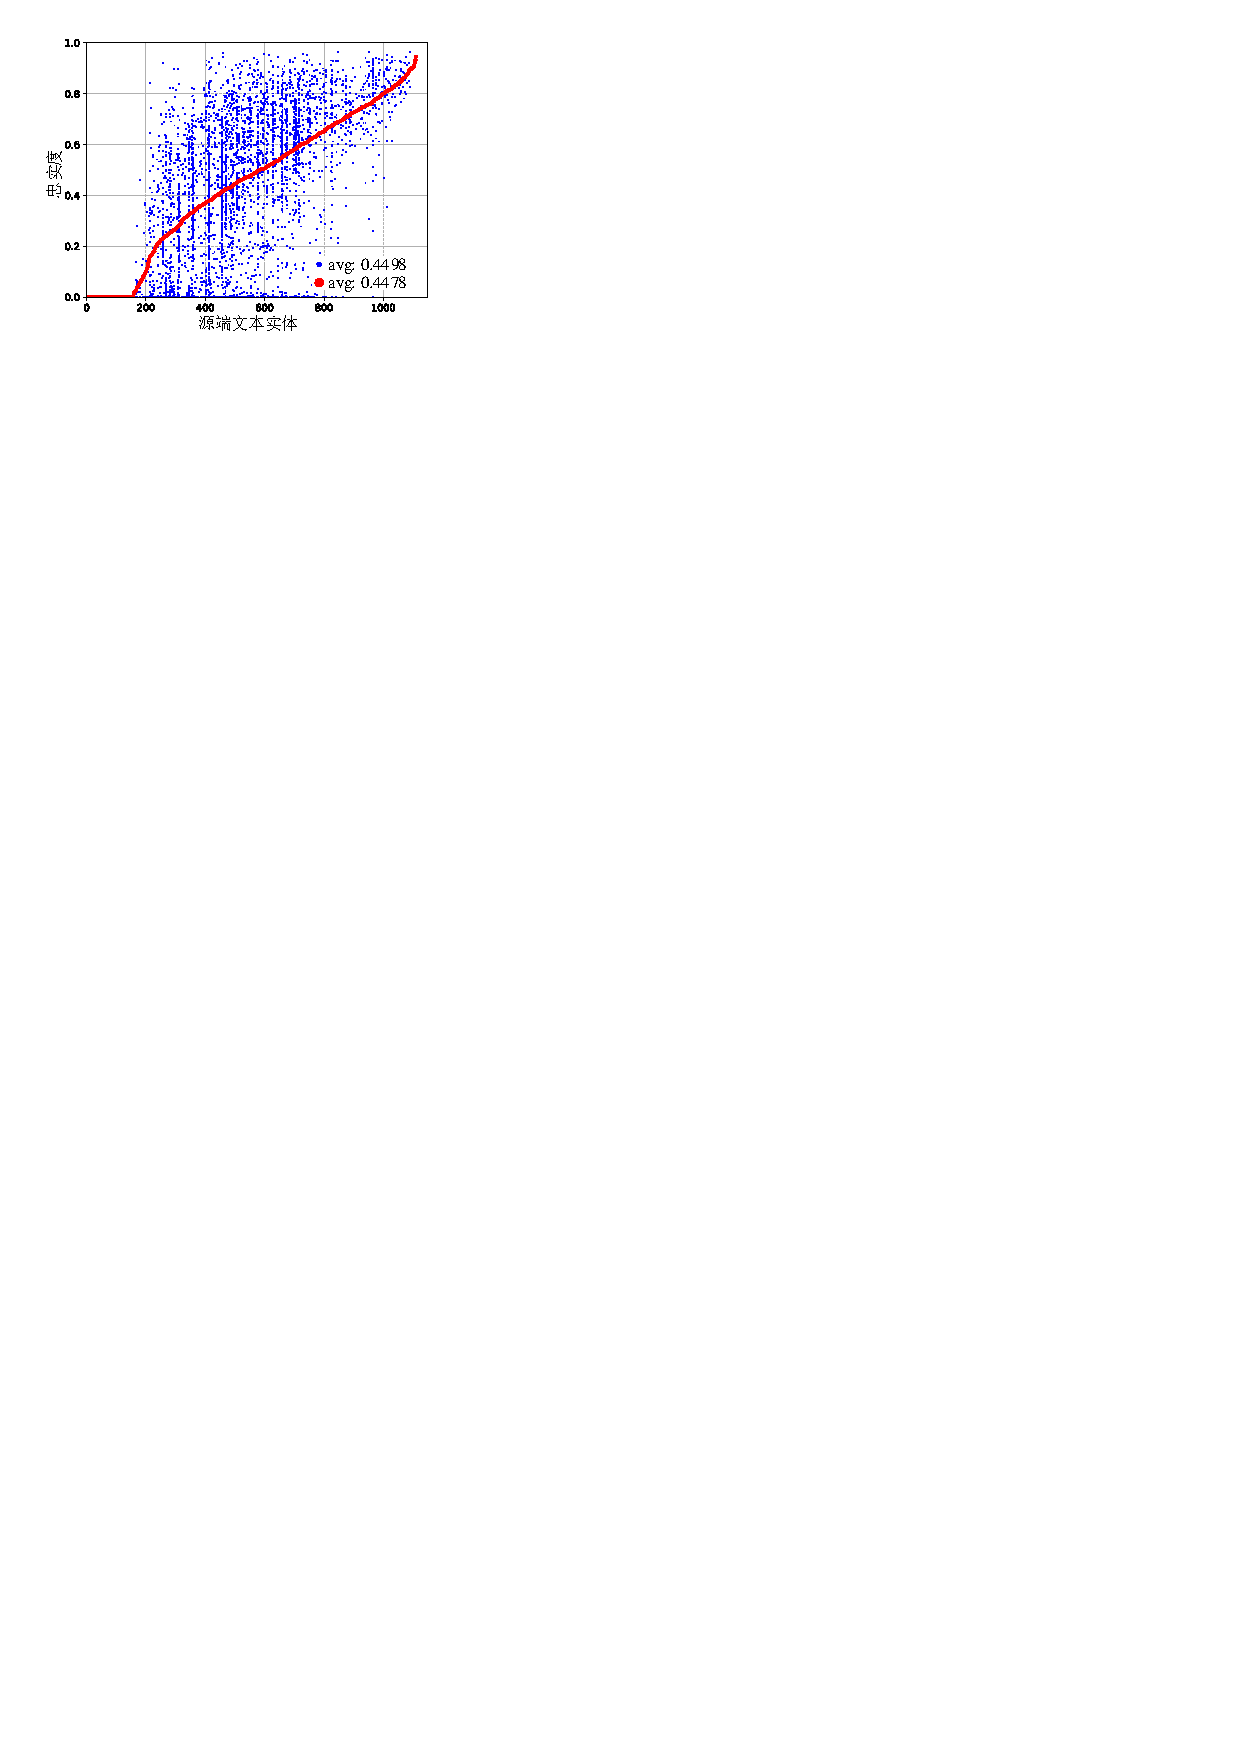
\includegraphics[width=\textwidth]{Img/fig_4_fidelity_cer_selforder.pdf}
      \caption{实体重排序的CER-NMT}
      \label{fig:4_fidelity_cer_selforder}
    \end{subfigure}%
    ~% add desired spacing
    \begin{subfigure}[b]{0.5\textwidth}
      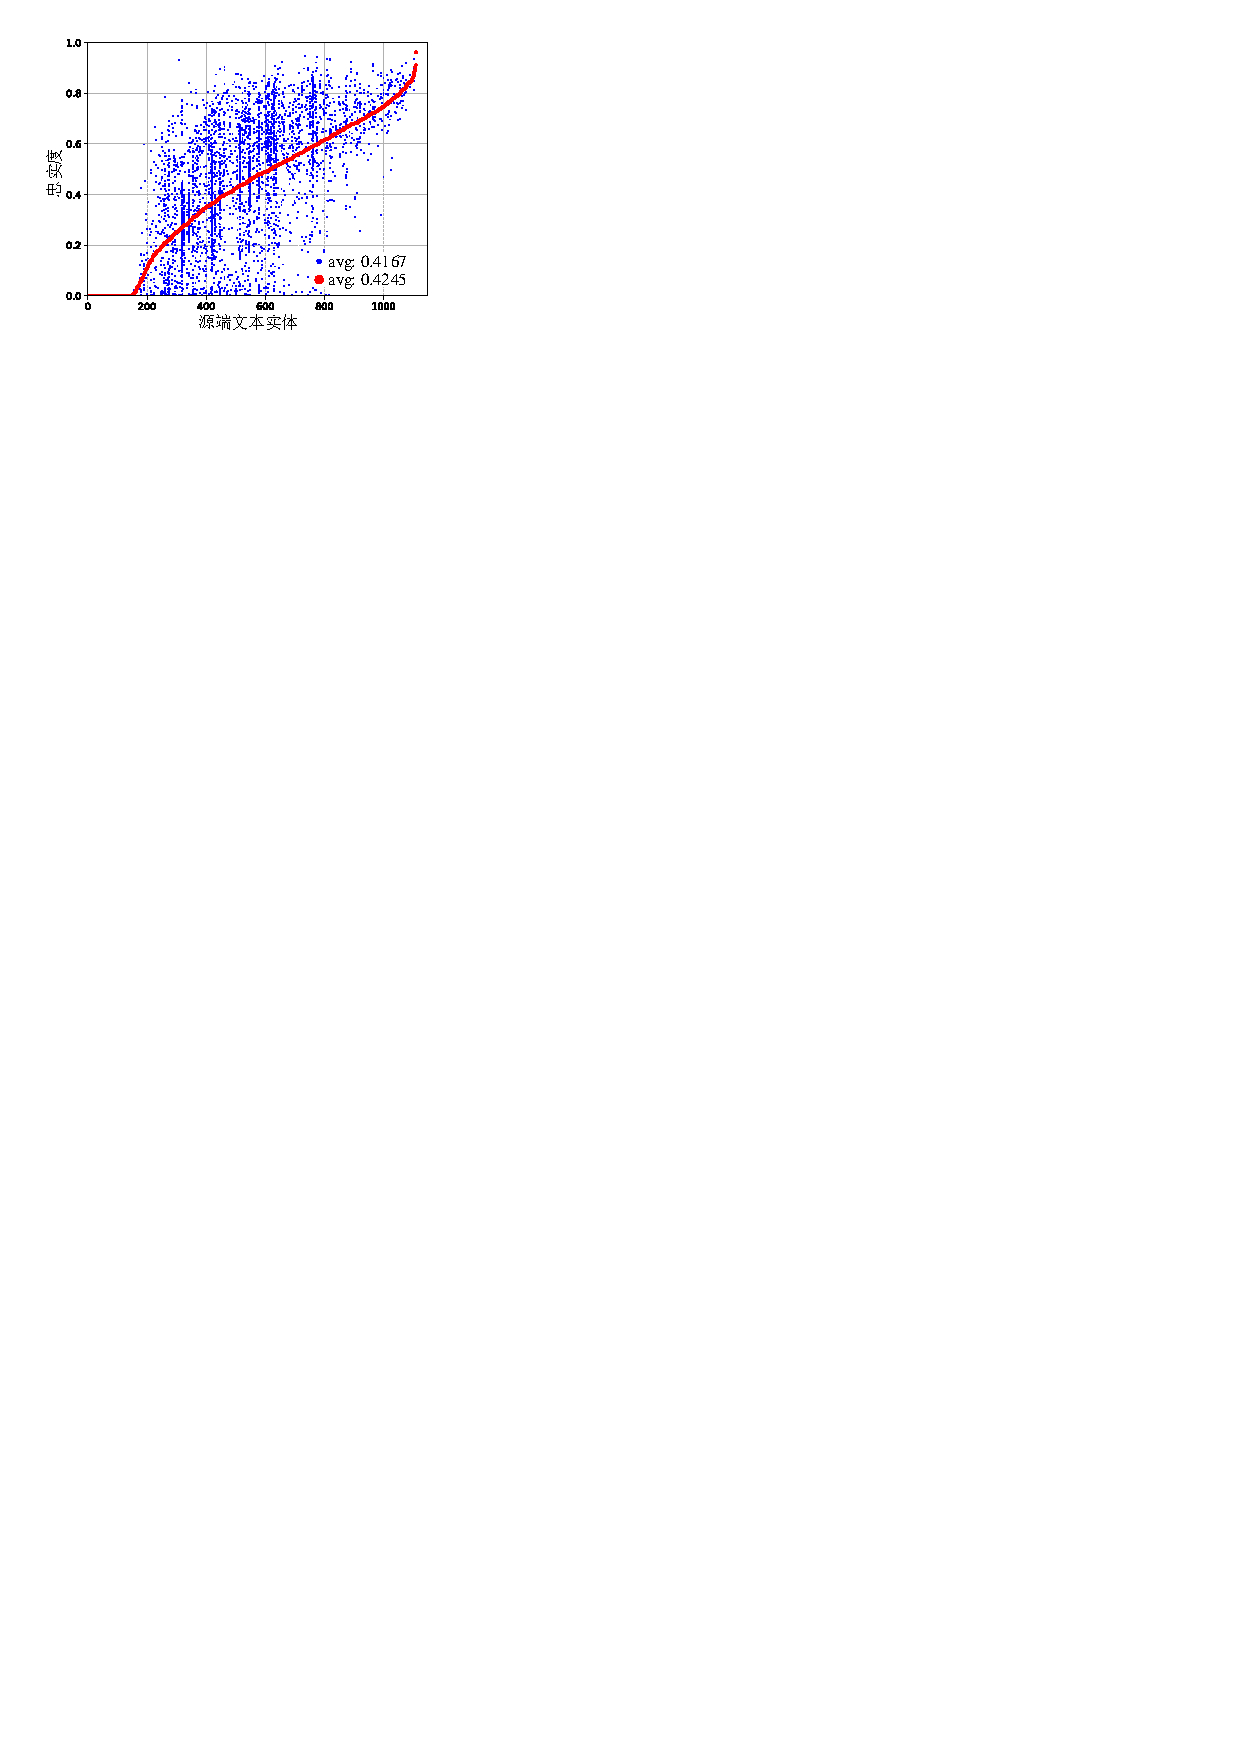
\includegraphics[width=\textwidth]{Img/fig_4_fidelity_tner.pdf}
      \caption{TNER-NMT}
      \label{fig:4_fidelity_tner}
    \end{subfigure}
    \bicaption{文本实体在不同模型下的忠实度}{The fidelity of textual entities on different models}
    \label{fig:4_fidelity}
\end{figure}
实验结果如图\ref{fig:4_fidelity}所示,图中横轴代表测试集中源语言文本实体以某种方式的排序,纵轴为范围从0到1的忠实度。每个小像素点代表一个源端文本实体在一个翻译句子样本中对应目标端文本实体的注意力权重值,即实体词忠实度。大圆点代表每个实体的平均忠实度。图\ref{fig:4_fidelity_base}为纯文本Transformer的测试结果,横轴为测试集中的1110个源端文本实体按照平均忠实度由小到大排序。图\ref{fig:4_fidelity_cer_baseorder}为CER-NMT与图\ref{fig:4_fidelity_base}横轴词序保持一致的结果,图\ref{fig:4_fidelity_cer_selforder}为CER-NMT对实体词重排序后的结果。图\ref{fig:4_fidelity_tner}为\ref{sec:4_ablation_study}节序号12仅设置TNER,且保持翻译任务训练比例不变的模型。图中“avg”代表平均值。从4个图的对比中可以得到以下信息:

%\item
(1)图中忠实度为0的横线部分代表对齐模型无法在目标端句子中找到对应的实体词。因此无法确定其忠实度。

%\item
(2)图\ref{fig:4_fidelity_cer_baseorder}相比于图\ref{fig:4_fidelity_base}存在更多靠近1.0的小像素点。从图\ref{fig:4_fidelity_cer_selforder}中的均值结果(avg)可以看到,小像素点的均值从0.4238提升至0.4498,大圆点的均值从0.4024提升至0.4478,均具有较明显的提升。该数值结果表明CER方法能够明显地提升模型在翻译过程中对源语言文本实体的忠实度。

%\item
(3)图\ref{fig:4_fidelity_cer_selforder}经过重排序实体的顺序后可以更直观地从曲线的趋势看出采用CER方法所带来的忠实度的提升。

%\item
(4)TNER对文本上下文和视觉实体进行句子级的语义融合,可以观察到图\ref{fig:4_fidelity_tner}相对于图\ref{fig:4_fidelity_base}有提升也有降低,这说明VER和TER才是帮助提升文本实体忠实度的主要因素,针对非实体的重构方法所带来的翻译性能提升无法没有显著地体现在实体忠实度的提升上。
%\end{itemize}

以上结果表明,CER方法通过融入视觉信息的方式,增加了翻译模型在翻译过程中对源语言文本实体的忠实度,从而使得翻译结果得到了进一步的提升。该实验同样表明本章的双向跨模态实体重构方法是有效可行的,该显式跨模态信息融合方法使得模型更具备可解释性,视觉信息的作用方式更有迹可循。